\documentclass[11pt, letterpaper]{article}

% ---- Packages ----
\usepackage[margin=1in, headheight=14pt]{geometry}
\usepackage{xcolor}
\usepackage{hyperref}
\usepackage{enumitem}
\usepackage{booktabs}
\usepackage{array}
\usepackage{colortbl}
\usepackage{tcolorbox}
\usepackage{fancyhdr}
\usepackage{titlesec}
\usepackage{parskip}
\usepackage[T1]{fontenc}
\usepackage{amsmath}
\usepackage{amssymb}
\usepackage{helvet}
\usepackage{pgfplots}
\pgfplotsset{compat=1.17}
\renewcommand{\familydefault}{\sfdefault}

% ---- Colors (Claude-inspired warm palette) ----
\definecolor{cprimary}{HTML}{C45A3C}      % warm terracotta
\definecolor{cdark}{HTML}{8B3A2A}         % deep burnt sienna
\definecolor{clight}{HTML}{FDF0E8}        % warm cream
\definecolor{cmedium}{HTML}{F5D5C3}       % soft peach
\definecolor{cdarktext}{HTML}{3D2B1F}     % warm dark brown
\definecolor{caccent}{HTML}{E8845A}       % coral accent
\definecolor{ctabhead}{HTML}{6B3422}      % dark table header

% ---- Hyperlink Setup ----
\hypersetup{
    colorlinks=true,
    linkcolor=cprimary,
    urlcolor=cprimary,
    citecolor=cprimary
}

% ---- Header / Footer ----
\pagestyle{fancy}
\fancyhf{}
\renewcommand{\headrulewidth}{0.4pt}
\renewcommand{\footrulewidth}{0.4pt}
\fancyhead[R]{\textit{\small\color{gray} PhD in Economics: Application Guide}}
\fancyfoot[C]{\small\color{gray} Page \thepage}

% ---- Section Formatting ----
\titleformat{\section}
  {\Large\bfseries\color{cdark}}
  {\thesection.}{0.5em}{}
  [\vspace{-0.5em}{\color{cprimary}\rule{\textwidth}{1.5pt}}]

\titleformat{\subsection}
  {\large\bfseries\color{cprimary}}
  {\thesubsection}{0.5em}{}

% ---- Tip Box ----
\newtcolorbox{tipbox}[1][]{
    colback=clight,
    colframe=cprimary,
    boxrule=0.5pt,
    leftrule=4pt,
    arc=0pt,
    fonttitle=\bfseries\color{cdark},
    title={#1},
    top=6pt, bottom=6pt, left=10pt, right=10pt
}

% ---- Contents Box ----
\newtcolorbox{contentsbox}{
    colback=clight,
    colframe=cdark,
    boxrule=1pt,
    arc=4pt,
    top=12pt, bottom=12pt, left=14pt, right=14pt
}

% ---- Document ----
\begin{document}
\color{cdarktext}

% ============= TITLE =============
\begin{center}
\colorbox{cdark}{%
\begin{minipage}[c]{0.92\textwidth}
\vspace{14pt}
\centering
{\Huge\bfseries\color{white} PhD in Economics and Finance}\\[8pt]
{\large\color{cmedium} Complete Application Guide for Prospective Students}\\[10pt]
{\normalsize\color{white} Niranjan Kumar (Olin School of Business) \& Claude}
\vspace{14pt}
\end{minipage}%
}
\end{center}

\vspace{12pt}

This guide consolidates key requirements, practical tips, and curated resources to help you navigate the PhD application process in economics.

\vspace{10pt}

\begin{contentsbox}
{\large\bfseries\color{cdark} Contents}
\vspace{6pt}

{\normalsize
\begin{enumerate}[leftmargin=*, itemsep=3pt, label={\color{cprimary}\bfseries\arabic*.}]
    \item \hyperref[sec:core]{Core Components of the Application Process: GRE, TOEFL, CV, SoP, LoR}
    \item \hyperref[sec:departments]{Choosing Economics Departments}
    \item \hyperref[sec:schoollist]{Building Your School List}
    \item \hyperref[sec:letterwriters]{Selecting Your Letter Writers}
    \item \hyperref[sec:diversity]{Diversity Statement and Personal Statement}
    \item \hyperref[sec:interviews]{Preparing for Interviews}
    \item \hyperref[sec:documents]{Documents Required:}
    \begin{enumerate}[label={\color{cprimary}\bfseries\arabic{enumi}.\arabic*.}, itemsep=2pt]
        \item \hyperref[sec:transcripts]{Transcripts and Grade Conversion}
        \item \hyperref[sec:coursework]{List of Related Coursework}
    \end{enumerate}
    \item \hyperref[sec:fees]{Application Fees and Fee Waivers}
    \item \hyperref[sec:appendix]{Appendix}
    \begin{enumerate}[label={\color{cprimary}\bfseries\arabic{enumi}.\arabic*.}, itemsep=2pt]
        \item \hyperref[sec:resources]{Curated Resources \& Further Reading}
        \item \hyperref[sec:checklist]{Final Application Checklist}
        \item \hyperref[sec:expenses]{Expense Tracker}
    \end{enumerate}
\end{enumerate}
}
\end{contentsbox}

\newpage

% ============= SECTION 1 =============
\section{Core Application Materials}\label{sec:core}

\subsection{Graduate Record Examination (GRE)}

Most top economics PhD programs require or strongly recommend the GRE General Test. The \textbf{Quantitative Reasoning} score is the most critical component. A strong quantitative score (166 and above) will put you in a competitive position at most programs. The Verbal and Analytical Writing sections matter (these are signals) for economics and still complement your overall profile.

\begin{itemize}[leftmargin=*, itemsep=2pt]
    \item A quantitative score of 166 or above is a solid benchmark. Prepare well and give yourself enough time to feel confident.
    \item Some programs have recently made the GRE optional. Always verify the current policy on each school's admissions page including the \textbf{cut-off.}
    \item Plan to take the test early enough to retake it if needed (scores are valid for 5 years).
\end{itemize}

\begin{tipbox}[Pro Tip]
Susan Athey notes that if you come from a university without strong faculty connections to top programs, objective criteria like GRE scores and grades in advanced math carry even greater weight in your application.
\end{tipbox}


\subsection{English Language Proficiency (TOEFL)}

International applicants whose native language is not English must submit proof of English proficiency. In the United States, the \textbf{TOEFL iBT} is by far the most widely accepted test, and many US economics PhD programs accept only the TOEFL. Aim for a score of 100 or above (some top programs prefer 105+).

\begin{itemize}[leftmargin=*, itemsep=2pt]
    \item Always check each program's admissions page to confirm which tests they accept. Also do not assume that alternatives like IELTS or Duolingo will be accepted.
    \item A small number of programs also accept IELTS Academic (typically requiring 7.0+ overall), but TOEFL remains the safest and most universally recognized option.
    \item Some programs waive the English proficiency requirement if you completed your undergraduate degree at an English-speaking institution.
\end{itemize}


\subsection{Letters of Recommendation}

Most programs require \textbf{three letters of recommendation}. These are among the most important components of your application. Strong letters come from faculty who know your academic work well and can speak to your research potential. Letters of Recommendation carry higher weight than other components.

\begin{enumerate}[leftmargin=*, itemsep=2pt]
    \item Choose recommenders who can speak specifically about your analytical abilities, intellectual curiosity, and capacity for independent research.
    \item At least two letters should ideally come from economics professors or researchers you have worked closely with.
    \item Letters that compare you to previous students who succeeded in top PhD programs are especially powerful.
    \item Ask yourself: does this person know my academic strengths and weaknesses? Also how closely have you worked with this person?
\end{enumerate}

\begin{tipbox}[Key Insight from Susan Athey]
Letters are most effective when recommenders explicitly compare you to other students they have seen succeed at top programs. This is especially critical if your professors do not have personal relationships with faculty at the schools you are applying to, as it helps the admissions committee calibrate the strength of their endorsement.
\end{tipbox}


\subsection{Statement of Purpose (SoP)}

Your statement of purpose should clearly articulate your research interests, relevant experience, and why a particular program is a good fit for you. This is your chance to demonstrate that you understand what graduate-level research entails.

\begin{itemize}[leftmargin=*, itemsep=2pt]
    \item Statement of Purpose is like storytelling. There is an arc to the story. Start with this question: what made you choose economics/finance research? How is your research experience an addition to your quest so far? Talk about your background and how a PhD program will shape you by sharing some of the ideas you plan to pursue during the PhD. Most likely you will end up doing something else than what you have written, but write some good research ideas.
    \item Describe your past research experience (thesis, RA work, summer projects) and connect it to your future research agenda.
    \item Name specific faculty members whose work aligns with your interests, but make sure your information is current and accurate.
    \item Show that you understand what a PhD involves: producing original research, not just taking classes.
    \item Keep it focused and concise (typically 1 to 2 pages).
\end{itemize}

\textbf{Note:} Economics admissions committees understand that research interests often change. The SoP is less about committing to a specific topic and more about demonstrating research maturity and intellectual seriousness.


\subsection{Curriculum Vitae (CV)}

Your academic CV should present a clear picture of your education, research experience, skills, and accomplishments. Unlike a job resume, an academic CV can be longer and more detailed.

\textbf{Key sections to include:}
\begin{itemize}[leftmargin=*, itemsep=2pt]
    \item Education (including relevant coursework in math and economics)
    \item Research experience (Pre-doc, RA Internships)
    \item Teaching experience (if applicable)
    \item Working papers
    \item Technical skills (programming languages: R, Stata, Python, MATLAB, etc.)
    \item Honors, awards, and fellowships
\end{itemize}

\begin{tipbox}[Working Papers: A Competitive Advantage]
While not required, having a working paper or a senior thesis that demonstrates original research can significantly strengthen your application. As Susan Athey notes, for applicants to top programs, an outstanding thesis can be a key differentiator, especially when paired with strong coursework and recommendations. If you have a co-authored paper with a faculty member, include it prominently.
\end{tipbox}


% ============= SECTION 2 =============
\section{Choosing Economics Departments}\label{sec:departments}

Choosing the right departments requires research beyond just looking at rankings. Here are some factors to consider.

\begin{itemize}[leftmargin=*, itemsep=2pt]
    \item \textbf{Faculty fit.} Look for departments with active faculty in your area of interest. Read their recent papers to see if their research excites you.
    \item \textbf{Placement record.} Check where recent graduates have been placed. A department with strong placements in your target career path (academia, policy, industry) is a good sign.
    \item \textbf{Program culture and size.} Smaller cohorts may offer more direct faculty interaction. Larger programs may offer more course variety and peer networks.
    \item \textbf{Funding and support.} Look into the funding packages offered to admitted students. Some programs guarantee funding for five or six years while others do not.
    \item \textbf{Location and cost of living.} Consider whether the stipend is adequate for the city where the program is located.
    \item \textbf{Talk to current students.} Reach out to current PhD students in departments you are considering. They can share honest perspectives on advising, workload, and culture.
\end{itemize}

\begin{tipbox}[Susan Athey's Advice on School Selection]
If you have a somewhat weaker record, there are lots of good graduate programs out there, but you need to shop more carefully for schools that have well-known advisors or have recently been investing a lot in graduate students. Some middle-ranked schools aggressively recruit prospective students and have placed graduating PhD students in top schools by investing heavily in the students. You need to do a lot of homework, and talk to lots of faculty about good places to apply.
\end{tipbox}

\newpage
% ============= SECTION 3 =============
\section{Building Your School List}\label{sec:schoollist}

There is no single right number, but here are some general guidelines.

\begin{itemize}[leftmargin=*, itemsep=2pt]
    \item Most applicants apply to \textbf{15 to 20 programs}. Applying to fewer than 15 is risky given how competitive admissions can be. I would personally recommend to apply 25 programs if you can do that.
    \item Create a normal curve: a few ``reach'' programs, several ``match'' programs where your profile fits well, and a couple of ``safety'' programs.
    \item Keep in mind that application fees add up. Budget for \$75 to \$150 per school and look into fee waivers early (see Section 8).
    \item Quality matters more than quantity. Tailor each Statement of Purpose rather than sending the same generic version to every school.
    \item Ask your recommenders and mentors for advice on your school list. Faculty who have served on admissions committees can help you calibrate where you are likely to be competitive.
\end{itemize}

\subsection{Why More Applications Help: The Probability Argument}

Each school makes its admissions decision independently. If your probability of acceptance at any single school is $p$, then the probability of getting \textit{at least one} acceptance from $n$ applications is:
$$P(\text{at least one}) = 1 - (1 - p)^{n}$$

The figure below shows how this probability grows as you apply to more schools for different per-school acceptance rates.

\begin{center}
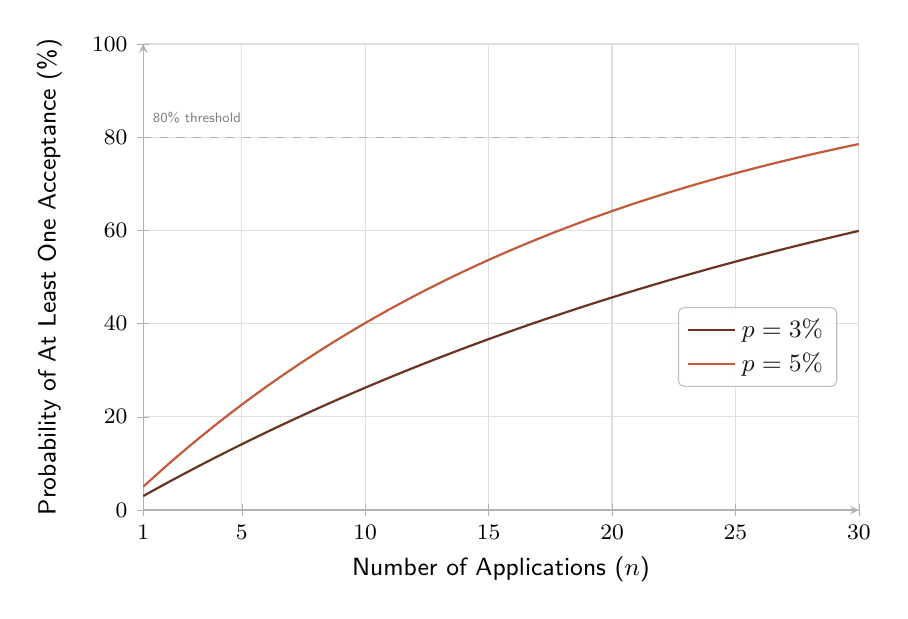
\begin{tikzpicture}
\begin{axis}[
    width=0.88\textwidth,
    height=7.5cm,
    xlabel={Number of Applications ($n$)},
    ylabel={Probability of At Least One Acceptance (\%)},
    xmin=1, xmax=30,
    ymin=0, ymax=100,
    xtick={1,5,10,15,20,25,30},
    ytick={0,20,40,60,80,100},
    grid=major,
    grid style={gray!25},
    legend style={
        at={(0.97,0.35)},
        anchor=east,
        font=\small,
        draw=gray!50,
        fill=white,
        fill opacity=0.9,
        rounded corners=2pt,
    },
    axis lines=left,
    every axis x label/.style={at={(0.5,-0.08)}, anchor=north, font=\small},
    every axis y label/.style={at={(-0.1,0.5)}, anchor=south, rotate=90, font=\small},
    axis line style={gray!60},
    tick style={gray!60},
    tick label style={font=\footnotesize},
]

% p = 3%
\addplot[
    color=ctabhead,
    thick,
    smooth,
    domain=1:30,
    samples=30,
] {100*(1 - (1-0.03)^x)};
\addlegendentry{$p = 3\%$}

% p = 5%
\addplot[
    color=cprimary,
    thick,
    smooth,
    domain=1:30,
    samples=30,
] {100*(1 - (1-0.05)^x)};
\addlegendentry{$p = 5\%$}

% Dashed reference at 80%
\addplot[
    dashed,
    gray!60,
    thin,
] coordinates {(1,80) (30,80)};

% Label for 80% line
\node[font=\tiny, gray, anchor=south west] at (axis cs:1,81) {80\% threshold};

\end{axis}
\end{tikzpicture}
\end{center}

This figure is just to give you an idea of acceptance rate. In reality, each school makes its decision independently. The probability of acceptance at any single school is going to change by school type.


% ============= SECTION 4 =============
\section{Selecting Your Letter Writers}\label{sec:letterwriters}

Your letters of recommendation can make or break your application. Choosing the right writers is just as important as what they say.

\begin{itemize}[leftmargin=*, itemsep=2pt]
    \item \textbf{Prioritize faculty who know your work.} A detailed letter from someone who has closely supervised your research is far more valuable than a generic letter from a famous professor.
    \item \textbf{Academic letters are preferred.} At least two of your three letters should come from academic economists or researchers. A third letter from an employer or policy supervisor can work if it speaks to your analytical skills.
    \item \textbf{Give your writers context.} Share your CV, SoP draft, and a summary of your school list so they can tailor their letters.
    \item \textbf{Ask early.} Give recommenders at least two months of notice before the deadline.
    \item \textbf{Follow up politely.} Recommenders are busy. A gentle reminder a week before the deadline is appropriate.
\end{itemize}

\begin{tipbox}[A Note for Students Without Strong Faculty Connections]
If you do not have relationships with economics professors (for example you are a math major) or if you attend a college without faculty connected to top PhD programs, you still have a good chance of admission if the rest of your application is strong. Be aware that objective criteria such as GRE scores, grades in hard math classes, and essays will receive more weight. Your professors' letters will be most effective if they compare you specifically to other students in top graduate programs.
\end{tipbox}


% ============= SECTION 5 =============
\section{Diversity Statement and Personal Statement}\label{sec:diversity}

Some programs ask for a \textbf{Diversity Statement} or a \textbf{Personal Statement} in addition to the Statement of Purpose. These are different documents with different goals.

\subsection{Diversity Statement}

\begin{itemize}[leftmargin=*, itemsep=2pt]
    \item This is your opportunity to share how your background, experiences, or identity contribute to diversity in the academic community.
    \item You do not need to belong to a specific demographic group to write a strong diversity statement. You can discuss overcoming challenges, unique perspectives you bring, or your commitment to creating inclusive environments.
    \item Keep it genuine. Admissions committees can tell when something feels forced.
\end{itemize}

\subsection{Personal Statement}

\begin{itemize}[leftmargin=*, itemsep=2pt]
    \item Some programs use the personal statement to learn about your motivations, life experiences, and how you arrived at the decision to pursue a PhD.
    \item Unlike the SoP (which focuses on research), the personal statement is more about you as a person.
    \item Not all programs require this. Check each application carefully and do not skip it if it is listed.
\end{itemize}


% ============= SECTION 6 =============
\section{Preparing for Interviews}\label{sec:interviews}

Not all economics PhD programs conduct interviews, but some do (especially for fellowship consideration or borderline candidates). Being prepared can only help.

Almost all finance departments, however, do conduct interviews. In general they try to gauge the candidate's interests, fit for the department, and their economic intuition. Expect questions about your research ideas, why you are drawn to finance, and how you think about economic problems. Treat it as a conversation rather than an exam.

\begin{itemize}[leftmargin=*, itemsep=2pt]
    \item \textbf{Know your CV and SoP inside out.} Be ready to discuss every research interest, project, and faculty name you mentioned.
    \item \textbf{Be ready to talk about your research.} If you have a thesis or working paper, practice explaining it clearly in 3 to 5 minutes.
    \item \textbf{Prepare questions for them.} Ask about advising style, the structure of the first year, placement support, or specific faculty research. This shows genuine interest.
    \item \textbf{Be honest about what you do not know.} It is perfectly fine to say you are still exploring your interests. Admissions committees value intellectual honesty.
    \item \textbf{Practice with peers or mentors.} A mock interview can help reduce anxiety and sharpen your responses.
\end{itemize}


% ============= SECTION 7 =============
\section{Documents Required}\label{sec:documents}

\subsection{Transcripts and Grade Conversion}\label{sec:transcripts}

All programs require official (or initially unofficial) transcripts from every undergraduate and graduate institution you have attended. When you submit your application, most schools accept uploaded copies, but upon admission you will be required to send official transcripts.

\subsubsection*{Grade Conversion for International Students}

If you studied outside the United States, your grading system may differ significantly. It is critical to ensure your grades are accurately converted or contextualized for U.S. admissions committees.

\vspace{6pt}
\begin{center}
\small
\renewcommand{\arraystretch}{1.4}
\begin{tabular}{>{\raggedright\arraybackslash}p{3cm} c c >{\raggedright\arraybackslash}p{4cm}}
\toprule
\rowcolor{ctabhead} \textcolor{white}{\textbf{Country / System}} & \textcolor{white}{\textbf{Scale}} & \textcolor{white}{\textbf{US Equiv.}} & \textcolor{white}{\textbf{Notes}} \\
\midrule
India (10-point)     & 8.0--10.0    & 3.5--4.0 GPA & Top marks in IITs/ISI carry strong weight \\
India (Percentage)   & 75--100\%    & 3.5--4.0 GPA & First Class with Distinction \\
\bottomrule
\end{tabular}
\end{center}
\vspace{6pt}

\begin{itemize}[leftmargin=*, itemsep=2pt]
    \item Consider using a credential evaluation service (WES, ECE, or SpanTran) to convert your grades to the US 4.0 scale.
    \item Some programs accept self-reported conversions while others require a formal evaluation.
    \item Always include a grading-scale explanation from your university if your transcript does not already contain one.
\end{itemize}


\subsection{List of Related Coursework}\label{sec:coursework}

Some applications ask you to list relevant coursework separately from your transcript. This is your chance to highlight the courses that matter most.

\begin{itemize}[leftmargin=*, itemsep=2pt]
    \item Include all math courses: calculus, linear algebra, real analysis, probability, statistics, differential equations.
    \item Include economics courses: intermediate micro and macro, econometrics, and any field courses.
    \item If you took graduate-level courses as an undergraduate, make sure to flag these clearly.
    \item List the grade received for each course if the application allows it.
\end{itemize}


% ============= SECTION 8 =============
\section{Application Fees and Fee Waivers}\label{sec:fees}

Application fees typically range from \$75 to \$150 per program, which can add up quickly if you are applying to 10 to 15 schools. Fortunately, many programs offer fee waivers.

\subsection{Common Eligibility Criteria for Fee Waivers}

\begin{itemize}[leftmargin=*, itemsep=2pt]
    \item Demonstrated financial hardship (often documented through FAFSA or financial aid records)
    \item Participation in recognized pipeline programs such as the AEA Summer Training Program (AEASP) or the AEA CSMGEP Mentoring Program
    \item U.S. McNair Scholars, TRIO, or similar federally funded programs
    \item Some schools grant waivers on a case-by-case basis upon request
\end{itemize}

\textbf{Important:} Fee waivers are often administered centrally by the Graduate School rather than the economics department. If you cannot find fee waiver information on the department website, contact the central graduate admissions office directly.

\subsection{The Economics Mentoring Program (EMP)}

\begin{tipbox}[About the EMP]
The Economics Mentoring Program (EMP), formerly known as AAMP, is a volunteer-based, student-run program that connects prospective PhD applicants with current graduate student mentors at \textbf{Berkeley, Harvard, MIT, Princeton, Stanford, and Yale.}

Mentors can provide advice on applications, feedback on materials, and insights into life as a PhD student. The program especially welcomes students with limited access to established networks and resources.

Applications for the 2026 cycle will open in mid-June 2026. Contact: economicsmentoring@gmail.com

\textbf{Website:} \href{https://www.economicsmentoringprogram.com/}{economicsmentoringprogram.com}
\end{tipbox}

\newpage

% ============= APPENDIX =============
\section{Appendix}\label{sec:appendix}

\subsection{Curated Resources \& Further Reading}\label{sec:resources}

The following resources are widely recommended by faculty, mentors, and successful applicants.

\subsubsection*{Application Advice and Mentorship Programs}

\begin{itemize}[leftmargin=*, itemsep=2pt]
    \item \textbf{Susan Athey, Professional Advice:} \href{https://gsb-faculty.stanford.edu/susan-athey/professional-advice/}{gsb-faculty.stanford.edu/susan-athey/professional-advice}
    \item \textbf{AEA/CSWEP Graduate School Resources:} \href{https://www.aeaweb.org/about-aea/committees/cswep/initiatives-and-resources/prof-dev-resources/grad-school}{aeaweb.org/cswep/grad-school}
    \item \textbf{Chris Blattman, PhD Application FAQ:} \href{https://chrisblattman.com/about/contact/gradschool/}{chrisblattman.com/gradschool}
    \item \textbf{Jesse Shapiro, Notes on Applying:} \href{https://scholar.harvard.edu/files/shapiro/files/phdnotes.pdf}{scholar.harvard.edu/shapiro}
    \item \textbf{EconGradAdvice (comprehensive resource compilation):} \href{https://sites.google.com/view/econgradadvice/}{sites.google.com/view/econgradadvice}
    \item \textbf{Extensive Guide for Applying to PhD Programs in Economics:} \href{https://drive.google.com/file/d/1cTb8enoUZxFKscidXYwojK3bXSjb7dxr}{Chakravorty, Kekre, Kundu, Narula \& Ojha}
    \item \textbf{Economics Mentoring Program (EMP):} \href{https://www.economicsmentoringprogram.com/}{economicsmentoringprogram.com}
    \item \textbf{AEA Summer Training Program (AEASP):} Intensive 2-month program in microeconomics, math, econometrics, and research methods.
\end{itemize}

\newpage
% ============= FINAL CHECKLIST =============
\subsection{Final Application Checklist}\label{sec:checklist}

\vspace{6pt}
\begin{center}
\renewcommand{\arraystretch}{1.6}
\begin{tabular}{c l c}
\toprule
\rowcolor{ctabhead} \textcolor{white}{\textbf{\checkmark}} & \textcolor{white}{\textbf{Item}} & \textcolor{white}{\textbf{Done}} \\
\midrule
\rowcolor{gray!8} $\square$ & GRE General Test (Quantitative, Verbal, AWA) & $\square$ \\
$\square$ & TOEFL (if applicable) & $\square$ \\
\rowcolor{gray!8} $\square$ & Three Letters of Recommendation & $\square$ \\
$\square$ & Statement of Purpose (tailored per school) & $\square$ \\
\rowcolor{gray!8} $\square$ & Diversity Statement / Personal Statement (if required) & $\square$ \\
$\square$ & Curriculum Vitae (CV) & $\square$ \\
\rowcolor{gray!8} $\square$ & Working Papers / Writing Sample (if available) & $\square$ \\
$\square$ & Transcripts (all institutions, with grade conversion if needed) & $\square$ \\
\rowcolor{gray!8} $\square$ & List of Related Coursework & $\square$ \\
$\square$ & List of faculty in each department with aligned interests & $\square$ \\
\rowcolor{gray!8} $\square$ & Application Fee Paid or Waiver Obtained & $\square$ \\
$\square$ & Verify Deadlines for Each Program & $\square$ \\
\bottomrule
\end{tabular}
\end{center}

\newpage
% ============= EXPENSE TRACKER =============
\subsection{Application Expense Tracker}\label{sec:expenses}

This is just a rough estimate of the cost of different components. I would recommend to create an expense tracker.

\vspace{6pt}
\begin{center}
\small
\renewcommand{\arraystretch}{1.5}
\begin{tabular}{>{\raggedright\arraybackslash}p{4.5cm} r r >{\raggedright\arraybackslash}p{3.5cm}}
\toprule
\rowcolor{ctabhead} \textcolor{white}{\textbf{Expense Item}} & \textcolor{white}{\textbf{Estimated Cost}} & \textcolor{white}{\textbf{Actual Cost}} & \textcolor{white}{\textbf{Notes}} \\
\midrule
\rowcolor{gray!8} GRE Registration & \$220 & & \\
GRE Score Sending (per school) & \$35 each & & \\
\rowcolor{gray!8} GRE Prep Materials & varies & & \\
TOEFL Registration & \$200--\$250 & & \\
\rowcolor{gray!8} TOEFL Score Sending (per school) & \$20 each & & \\
Application Fees (per school) & \$75--\$150 each & & \\
\rowcolor{gray!8} Credential Evaluation (WES/ECE) & \$100--\$250 & & \\
Transcript Requests & \$5--\$25 each & & \\
\rowcolor{gray!8} Postage / Mailing Costs & varies & & \\
Interview Travel (if applicable) & varies & & \\
\midrule
\rowcolor{clight} \textbf{Total (estimated for 10 schools)} & \textbf{\$1,500--\$2,500+} & & \\
\bottomrule
\end{tabular}
\end{center}
\vspace{6pt}

\begin{tipbox}[Budget Tip]
Start looking into fee waivers early. Between GRE, TOEFL, and application fees alone, applying to 10 to 15 schools can easily exceed \$2,000. Many of these costs can be reduced or eliminated with fee waivers and score-sending offers.
\end{tipbox}

\vspace{20pt}

% ============= CLOSING =============
\begin{center}
\colorbox{cmedium}{%
\begin{minipage}[c]{0.85\textwidth}
\vspace{10pt}
\centering
{\large\bfseries\color{cdark} Good luck with your applications!}\\[6pt]
{\normalsize Start early, seek feedback, and remember that the application is just the beginning of your research journey.}
\vspace{10pt}
\end{minipage}%
}
\end{center}

\end{document}
